\documentclass[a4paper,12pt]{report}
\setcounter{secnumdepth}{5}
\setcounter{tocdepth}{3}
\input{/usr/share/LaTeX-ToolKit/template.tex}
\begin{document}
\title{Euclidean Geometry}
\author{沈威宇}
\date{\temtoday}
\titletocdoc
\ch{Euclidean Geometry (歐幾里德幾何學)}
\ssc{Plane angle (平面角) or angle}
\sssc{Degree, deg, degree of arc, arc degree, or arcdegree (角度)}
One degree, deg, degree of arc, arc degree, or arcdegree, denoted as $^\circ$, is defined such that one full revolution is 360 degrees.

One degree is divided into 60 minutes, minutes of arc, arc minutes, or arcminutes, denoted as a single prime $'$, and one minute is divided into 60 seconds, seconds of arc, arc seconds, or arcseconds, denoted as a double prime $"$.
\sssc{Radian or rad (弧度, 弳, 弳度)}
One radian or rad, denoted as rad or without suffix, is defined as the angle subtended at the center of a unit circle by an arc of unit length, that is $\frac{180}{\pi}^\circ$.
\sssc{Gradian, grad, or gon}
One gradian, grad, or gon, denoted as grad, is defined as $0.9^\circ$.
\sssc{Milliradian, mrad, or mil}
A milliradian, mrad, or mil, denoted as mrad, is defined as $\frac{1}{1000}$ radian.
\sssc{Turn, tr, pla, revolution, rev, cycle, or cyc}
One turn, tr, pla, revolution, rev, cycle, or cyc is defined as $360^\circ$.
\sssc{Generalized angle (廣義角) or directed angle (有向角)}
A generalized angle or directed angle is an angle of any real number with positive value denotes counterclockwise angle and negative value denotes clockwise angle.

Two directed angles are coterminal angles (同界角) if their difference is $2k\pi$ radians with $k\in\bbR$.
\sssc{三角測量}
\begin{itemize}
\item \tb{仰角(angle of elevation)}:仰視目標時,視線與水平線的夾角。
\item \tb{俯角(angle of depression)}:俯視目標時,視線與水平線的夾角。
\item \tb{高度角(altitude angle)}:仰視目標時,即仰角;平視目標時,為零;俯視目標時,即負一乘以俯角。
\item \tb{天頂角(zenith angle)/傾(斜)角(inclination)}:90$^{\circ}$減去高度角。
\item \tb{方位角(azimuth or azimuthal angle)}(地理):以正北為0$^\circ$,順時針為正。
\item \tb{象限角(reduced bearing)}(地理):以東南西北某一方位(通常為正北或正南) 為基準,加上向相鄰方位轉向的度數與該相鄰方位,如北35$^\circ$西 代表方位角325$^\circ$、南30$^\circ$西代表方位角210$^\circ$。
\end{itemize}
\ssc{Solid angle (立體角)}
\sssc{Steradian, square radian, or sr (球面度 or 立弳)}
One steradian, square radian, or sr, denoted as sr, is defined as the solid angle subtended at the centre of a unit sphere by a unit area (of any shape) on its surface.
\sct{二維形狀}
\ssc{多邊形}
\sssc{多邊形內角和公式}
任二邊不相交於該二邊之頂點(如有)以外之處的$n$邊形,其內角和為$(n-2)\pi$。
\ssc{三角形}
令圖形體積(或面積、長度)之代號同其自身。今有一三角形$\Delta ABC$,其中:$\angle A$、$\angle B$、$\angle C$的對邊長分別為$a$、$b$、$c$;$\angle A$、$\angle B$、$\angle C$又記作$A$、$B$、$C$;重心$G$;外接圓$O$圓心$O$即外心、半徑$R$;內接圓$I$圓心$I$即內心、半徑$r$;垂心$H$;$\angle A$、$\angle B$、$\angle C$的對邊中點分別為$M_a$、$M_b$、$M_c$;$A$在$\olra{BC}$的垂足為$h_a$,$B$在$\olra{CA}$的垂足為$h_b$,$C$在$\olra{AB}$的垂足為$h_c$;$s=\frac{1}{2}\qty(a+b+c)$;$\angle A$、$\angle B$、$\angle C$的角平分線與對邊之交點分別為$\mathscr{B}_a$、$\mathscr{B}_b$、$\mathscr{B}_c$;九點圓$\mathscr{O}$圓心$\mathscr{O}$、半徑$\mathscr{R}$;與$A$、$B$、$C$的兩鄰邊延長線與對邊皆相切的旁切圓分別為$E_a$、$E_b$、$E_c$,其圓心(旁心)各同其圓名。
\sssc{勾股/商高/畢氏定理(Pythagorean theorem or Pythagoras' theorem)}
\[(\angle C=90^\circ)\iff (a^2+b^2=c^2)\]
\begin{proof}\mbox{}\\
趙爽勾股圓方圖證明法:
\begin{center}
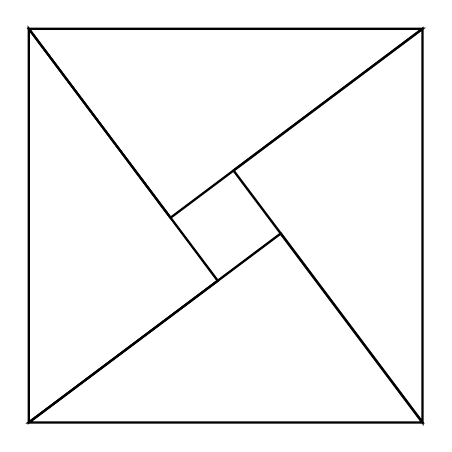
\begin{tikzpicture}
\draw[thick] (0,0) -- (16/5,12/5) -- (5,0) -- cycle;
\draw[thick] (0,0) -- (12/5,9/5) -- (0,5) -- cycle;
\draw[thick] (0,5) -- (5,5) -- (9/5,13/5) -- cycle;
\draw[thick] (5,0) -- (13/5,16/5) -- (5,5) -- cycle;
\end{tikzpicture}
\end{center}
其中四個三角形的短股為$a$、長股為$b$、斜邊為$c$。
\[4\frac{ab}{2}+(b-a)^2=c\]
\[a^2+b^2=c^2\]
\end{proof}
\sssc{三角形全等與$SSA$型性質}
令:已知兩三角形一對應位置之邊長相等稱$S$,已知兩三角形一對應位置之角之角度相等稱$A$,$S$相鄰表示鄰邊,$A$相鄰表示鄰角,$S$與$A$相鄰表示邊與其一側的角,當$A$為直角得稱$R$,$R$之鄰邊得稱$H$。

三角形的全等性質有$SSS$、$SAS$、$AAS$、$ASA$、$RHS$,當兩三角形符合以上任一條件時,知兩三角形全等。

$SSA$型的討論:若已知$a$、$b$、$\angle A$:
\begin{itemize}
\item $\angle A$為銳角,因$C$到$\olra{AB}$的距離為$b\sin A$:
\begin{itemize}
\item $a<b\sin A$: 無解
\item $a=b\sin A$: 唯一解
\item $a>b\sin A$: 兩解
\end{itemize}
\item $\angle A$為鈍角,則:
\begin{itemize}
\item $a\leq b$: 無解
\item $a>b$: 唯一解
\end{itemize}
\end{itemize}
\sssc{九點圓(Nine-point circle)/歐拉圓(Euler's circle)/費爾巴哈圓(Feuerbach circle)與歐拉線(Euler line)}
\bit
\item $M_a,M_b,M_c,h_a,h_b,h_c,\frac{A+H}{2},\frac{B+H}{2},\frac{B+H}{2}$必共圓,該圓稱九點圓(Nine-point circle)、歐拉圓(Euler's circle)或費爾巴哈圓(Feuerbach circle)。
\item 九點圓圓周$\mathscr{O}$與圓心$\mathscr{O}$均符合:
\[\mathscr{O}=\frac{O+H}{2}\]
\item $\mathscr{O},O,G,H$必共線,該線稱歐拉線(Euler line)。
\item $\Delta ABC$ 是等腰三角形 $\iff I$ 在歐拉線上。
\item 費爾巴哈定理(Feuerbach's theorem):九點圓與三個旁切圓均外切,與內切圓內切(內切圓在內)。
\item \[\mathscr{R}=\frac{R}{2}\]
\eit
\sssc{正弦定理(Law of sines)}
\[\frac{\sin A}{a}=\frac{\sin B}{b}\]
\begin{proof}
\[\sin A=\frac{\overline{Ch_c}}{a}\]
\[\sin B=\frac{\overline{Ch_c}}{b}\]
\end{proof}
\[2R\sin A =a\]
\begin{proof}\mbox{}\\
作$O$。若$\Delta ABC$為直角三角形,觀察可證。若$\Delta ABC$非直角三角形,以$BC$為一股,令斜邊在$\olra{BO}$上,作一直角三角形$BCD$,其中$D=2O-B$。若$\Delta ABC$為銳角三角形,根據圓周定理可知,$\angle D = \angle BAC$,得證。若$\Delta ABC$為鈍角三角形,根據根據圓內接四邊形對角互補定理可知,$\angle D = \pi- \angle A$,得證。
\end{proof}
\sssc{凸四邊形面積公式}
\[\text{凸四邊形面積=$\frac{1}{2}$對角線相乘$\times\sin$兩對角線夾角}\]
\sssc{投影定理}
\[a=b\cos C+c\cos B\]
\sssc{餘弦定理(Law of cosines)}
\[a^2=b^2+c^2-2bc\cos A\]
\begin{proof}\mbox{}\\
根據投影定理:
\[c=a\cos B+b\cos A\]
兩邊同乘$c$:
\[c^2=ac\cos B +bc\cos A\]
同理:
\[a^2=ac\cos B +ab\cos C\]
\[c^2=bc\cos A +ab\cos C\]
\[c^2=a^2-ab\cos C+b^{2}-ab\cos C=a^{2}+b^{2}-2ab\cos C\]
\end{proof}
\sssc{平行四邊形邊長與對角線長平方公式}
\[\text{平行四邊形四邊長平方和等於兩對角線長平方和}\]
\sssc{三角形中線公式}
\[\overline{AB}^2+\overline{AC}^2=2\qty(\overline{AM_a}^2+\overline{BM_a}^2)\]
\sssc{三角形面積公式}
\bma
\Delta ABC &= \frac{1}{2}a\cdot \ol{Ah_a}\\
&= \frac{1}{2}ab\sin C\\
&= \sqrt{s(s-a)(s-b)(s-c)}\quad\text{(海龍(Heron)公式)}\\
&= \frac{abc}{4R}\\
&= rs\\
&= \frac{1}{\sqrt{\qty(\frac{1}{h_a}+\frac{1}{h_b}+\frac{1}{h_c})\qty(-\frac{1}{h_a}+\frac{1}{h_b}+\frac{1}{h_c})\qty(\frac{1}{h_a}-\frac{1}{h_b}+\frac{1}{h_c})\qty(\frac{1}{h_a}+\frac{1}{h_b}-\frac{1}{h_c})}}\\
&= \frac{2}{3}\ol{BM_b}\cdot \ol{CM_c}\sqrt{\qty|\frac{1-\qty(\ol{AM_a}^2+\ol{BM_b}^2+\ol{CM_c}^2)^2}{4\ol{BM_b}^2\ol{CM_c}^2}|}\\
&= \frac{1}{2}\sqrt{\ol{AB}^2\ol{AC}^2-\qty(\ora{AB}\cdot \ora{AC})^2}\\
&= \frac{1}{2}\abs{\abs{\ora{AB}\times \ora{AC}}}
\eam
\sssc{重心(Centroid)}
\[G\tx{\ 為三中線交點}\]
\[\ora{AG}=2\ora{GM_A}\]
\[G=\frac{A+B+C}{3}\]
\[\ora{GA}+\ora{GB}+\ora{GC}=\ora{0}\]
\[\Delta GAB=\Delta GAC=\Delta GBC\]
\sssc{外心(Circumcenter)相關定理}
\[\ol{OA}=\ol{OB}=\ol{OC}=R\]
\[O=\frac{a^2A+b^2B+c^2C}{a^2+b^2+c^2}\]
\[O\tx{\ 為三邊中垂線交點}\]
\[\Delta OAB : \Delta OBC : \Delta OCA = \sin 2C : \sin 2A : \sin 2B\]
\[ \ora{AO}\cdot \ora{AB} = \frac{1}{2}\ol{AB}^2 \]
\[\frac{1}{2}\angle AOB = \angle C\lor\pi -\angle C\]
\sssc{內心(Incenter)}
\[I\tx{\ 與三邊均相切}\]
\[I\tx{\ 為三角角平分線交點}\]
\[I=\frac{aA+bB+cC}{a+b+c}\]
\[a\ora{IA}+b\ora{IB}+c\ora{IC}=\ora{0}\]
\[\Delta IAB : \Delta IBC : \Delta ICA = c : a : b\]
\sssc{垂心(Orthocenter)}
\[H\tx{\ 為三高交點}\]
\[H=\frac{\tan A\cdot A+\tan B\cdot B+\tan C\cdot C}{\tan A+\tan B+\tan C}\]
\[ \ora{AH}\cdot\ora{AB}=\ora{AH}\cdot\ora{AC}=\ora{AB}\cdot\ora{AC}=\frac{1}{2}\qty(\ora{AC}^2+\ora{AB}^2-\ora{BC}^2)\]
\[\tx{在複數平面上:}
\det \begin{pmatrix} 1 & A & A^2 & \overline A \\
1& B & B^2 & \overline B \\
1& C & C^2 & \overline C \\
1& H & H^2 & \overline H
\end{pmatrix}=0\]
\[\frac {\overline {Hh_a}}{\overline {Ah_a}}+\frac {\overline {Hh_b}}{\overline {Bh_b}}+\frac {\overline {Hh_c}}{\overline {Ch_c}}=1\]
\sssc{西瓦定理(Ceva theorem)}
令西瓦線段指各頂點與其對邊或對邊延長線連接而成的直線段。
\bma
& \text{三角形$\Delta ABC$的西瓦線段$\ora{AD}$、$\ora{BE}$、$\ora{CF}$:}\\
& \tx{$\ora{AD}$、$\ora{BE}$、$\ora{CF}$ 交於一點} \iff \frac {\overline {BD}}{\overline {DC}}\cdot \frac {\overline {CE}}{\overline {EA}}\cdot \frac {\overline {AF}}{\overline {FB}}=1 \implies D\tx{、}E\tx{、}F\tx{中有零或二個點不在 }\Delta ABC\tx{\ 邊上}
\eam
口訣:頂分頂分頂分頂
\sssc{孟氏定理(Menelaus' theorem)}
\bma
& \text{一直線與${\displaystyle \Delta ABC}$的邊$BC$、$CA$、$AB$或其延長線分別交於$L$、$M$、$N$}\\
& \iff \frac {\overline {AN}}{\overline {NB}}\cdot \frac {\overline {BL}}{\overline {LC}}\cdot \frac {\overline {CM}}{\overline {MA}}=1 \implies L\tx{、}M\tx{、}N\tx{中有一或三個點不在 }\Delta ABC\tx{\ 邊上}
\eam
口訣:頂分頂分頂分頂
\sssc{角平分線定理}
已知:$\Delta ABC$中$\angle B$<$\angle C$;$D$在$\ol{BC}$上;$E$在$\ora{BC}$上且不在$\ol{BC}$上。

內角平分線定理及逆定理:
\[\angle BAD =\angle DAC \Leftrightarrow {\frac {\ol{DB}}{\ol{DC}}}={\frac {\ol{AB}}{\ol{AC}}}\]
外角平分線定理及逆定理:
\[\angle CAE =\pi-\angle BAE \Leftrightarrow {\frac {\ol{EB}}{\ol{EC}}}={\frac {\ol{AB}}{\ol{AC}}}\]
\sssc{角平分線長定理}
\[\ol{A\mathscr{B}_a}=\frac{bc\sin A}{\qty(b+c)\sin\qty(\frac{A}{2})}\]
\ssc{圓上圖形}
\sssc{圓內二弦夾角公式}
圓心$O$之圓內二弦$\ol{AB}$、$\ol{CD}$交於$E$,則:
\[\angle AEC=\frac{1}{2}\qty(\angle AOC+\angle BOD)\]
當$B=D=E$:
\[\angle AEC=\frac{1}{2}\angle AOC\]
當$B=D=E$且$\ol{AC}$為一直徑:
\[\angle AEC=\frac{\pi}{2}\]
\sssc{圓內接四邊形公式}
一圓內接四邊形$ABCD$,$\ol{AB}=a$、$\ol{BC}=b$、$\ol{CD}=c$、$\ol{DA}=d$:
\[\angle A+\angle C=\pi\]
\[\ol{AC}^2=\frac{\qty(ac+bd)\qty(ad+bc)}{ab+cd}\]
\[\ol{BD}^2=\frac{\qty(ac+bd)\qty(ad+cd)}{ad+bc}\]
\[\ol{AC}\cdot\ol{BD}=ac+bd\]
\ssc{球面}
\sssc{球面餘弦定律}
空間中與一定點 $O$ 距離為 $R>0$ 的所有點 $P$ 所形成的圖形稱一球面,其中 $O$ 稱為球心,$R$ 稱為半徑。

令球面上有球面三角形$ABC$,$\angle A$之對邊弧長除以球面之半徑等於$a$,$\angle B$之對邊弧長除以球面之半徑等於$b$,$\angle C$之對邊弧長除以球面之半徑等於$c$。

第一球面餘弦定律:
\[\cos c = \cos a \cos b + \sin a \sin b \cos C\]
第二球面餘弦定律/角度餘弦定律:
\[\cos C = - \cos A \cos B + \sin A \sin B \cos c\]
\sct{三維形狀}
\ssc{各體公式}
\[\tx{柱體體積}=\tx{底面積}\times \tx{高}\]
\[\tx{錐體體積}=\frac{1}{3}\tx{底面積}\times \tx{高}\]
\[\tx{球體體積}=\f{4}{3}\pi\times\tx{半徑}^3\]
\[\tx{球體表面積}=4\pi\times\tx{半徑}^2\]
\ssc{四面體}
\sssc{正四面體}
正四面體A-BCD邊長 $a$,高 $h$,表面積 $A$,體積 $V$,外接球半徑 $R$,內接球半徑 $r$,$\olra{AB}$與$\olra{CD}$距離 $s$,重心 $\frac{A+B+C+D}{4}$與$A$的距離 $g$:
\[h=\frac{\sqrt{6}}{3}a\]
\[A=\sqrt{3}a^2\]
\[V=\frac{\sqrt{2}}{12}a^3\]
\[R=\frac{\sqrt{6}}{4}a\]
\[r=\frac{\sqrt{6}}{12}a\]
\[s=\frac{\sqrt{2}}{2}a\]
\[g=\frac{\sqrt{6}}{4}a\]
\sssc{四面體內接球半徑定理}
\[\tx{內接球半徑}=\frac{3\cdot\tx{體積}}{\tx{表面積}}\]
\sct{Coordinate System (座標系)}
\ssc{極座標系(Polar Coordinate System)}
極座標系是由一參考點,稱極點(pole)或原點(origin),與一始於極點的射線,稱極軸(polar axis),定義的二維座標系。令一個點在以極點為原點、極軸為$x$軸正向的二維右手笛卡爾座標系中有座標$(r\cos\theta,r\sin\theta)$使得$r\geq 0\land\theta\in[0,2\pi)$,則該點在此極座標系中有極座標$(r;\theta)$,其中$r$稱徑向距離(radial distance or radius),即與原點的距離,$\theta$稱極角(polar angle),即相對於$x$軸、逆時針增加的角位置。
\ssc{球座標系(Spherical Coordinate System)}
\sssc{ISO 80000-2:2019/物理慣例(physics convention)/傾斜角、方位角的球座標系}
ISO 80000-2:2019/物理慣例/傾斜角、方位角的球座標系是由一參考點,稱原點(origin),一始於原點的射線,稱極軸(polar axis),與一包含極軸的平面,稱初始子午面(initial meridian plane),定義的三維座標系。令一個點在以原點為原點、極軸為$z$軸正向、初始子午面為$xz$平面的三維右手笛卡爾座標系中有座標$(r\sin\theta\cos\varphi,r\sin\theta\sin\varphi,r\cos\theta)$使得$r\geq 0\land\theta\in[0,\pi]\land\varphi\in[0,2\pi)$,則該點在此球座標系中有球座標$(r;\theta;\varphi)$,其中$r$稱徑向距離(radial distance or radius),即與原點的距離,$\theta$稱傾(斜)角(inclination)、極角(polar angle)或天頂角(zenith angle),即與$z$軸正向的夾角,$\varphi$稱方位角(azimuth or azimuthal angle),即在$xy$平面正射影相對於$x$軸、逆時針增加的角位置。
\sssc{方位角、高度角的球座標系}
方位角、高度角的球座標系是由一參考點,稱原點(origin),一始於原點的射線,稱極軸(polar axis),與一包含極軸的平面,稱初始子午面(initial meridian plane),定義的三維座標系。令一個點在以原點為原點、極軸為$z$軸正向、初始子午面為$xz$平面的三維右手笛卡爾座標系中有座標$(r\cos\varphi\cos\theta,r\cos\varphi\sin\theta,r\sin\varphi)$使得$r\geq 0\land\theta\in[0,2\pi)\land\varphi\in(-\frac{\pi}{2},\frac{\pi}{2})$,則該點在此球座標系中有球座標$(r;\theta;\varphi)$,其中$r$稱徑向距離(radial distance or radius),即與原點的距離,$\theta$稱方位角(azimuth or azimuthal angle),即在$xy$平面正射影相對於$x$軸、逆時針增加的角位置,$\varphi$稱高度角(altitude angle)或仰角(angle of elevation),即相對於在$xy$平面正射影、逆時針增加的角位置,即$\frac{\pi}{2}$減去高度角。
\sssc{高度角、方位角的球座標系}
高度角、方位角的球座標系是由一參考點,稱原點(origin),一始於原點的射線,稱極軸(polar axis),與一包含極軸的平面,稱初始子午面(initial meridian plane),定義的三維座標系。令一個點在以原點為原點、極軸為$z$軸正向、初始子午面為$xz$平面的三維右手笛卡爾座標系中有座標$(r\cos\theta\cos\varphi,r\cos\theta\sin\varphi,r\sin\theta)$使得$r\geq 0\land\theta\in(-\frac{\pi}{2},\frac{\pi}{2})\land\varphi\in[0,2\pi)$,則該點在此球座標系中有球座標$(r;\theta;\varphi)$,其中$r$稱徑向距離(radial distance or radius),即與原點的距離,$\theta$稱高度角(altitude angle)或仰角(angle of elevation),即相對於在$xy$平面正射影、逆時針增加的角位置,即$\frac{\pi}{2}$減去高度角,$\varphi$稱方位角(azimuth or azimuthal angle),即在$xy$平面正射影相對於$x$軸、逆時針增加的角位置。
\sct{Analytic Geometry (解析幾何)}
下:空間為歐幾里德空間;位置$\mathbf{x}=(x_1,x_2,\ldots)$;第$i$軸正方向單位向量$\mathbf{e}_i$;一向量空間中兩點$P$、$Q$,$\ora{PQ}\coloneq Q-P$;$\hat{\mathbf{v}}$為$\mathbf{v}$正方向單位向量。
\ssc{正整數維空間}
$n\in\mathbb{N}$
\sssc{仿射子空間一般式}
$\mathbb{R}^n$中,一$n-1$維仿射子空間可以表示成:
\[\mathbf{n}\cdot\mathbf{x}+c=0\]
稱此表達方法為一般式。
\sssc{仿射子空間截距式}
$\mathbb{R}^n$中,$n-1$維仿射子空間:
\[E\colon\sum_{i=1}^n\frac{x_1}{a_1}=1\]
必通過$a_i\mathbf{e}_i$,$\forall i\in\mathbb{N}\land i\leq n$,稱此表達方法為截距式,稱$a_i$為第$i$軸截距。
\sssc{仿射子空間隱式方程/多面式}
$\mathbb{R}^n$中,一個$m\in\mathbb{N}\land m<n$維仿射子空間$E$可表示成:
\[\mathbf{A}\mathbf{x}=\mathbf{c},\quad\mathbf{A}\in\mathbb{R}^{(n-m)\times n}\land\operatorname{rank}(\mathbf{A})=n-m\land\mathbb{c}\in\mathbb{R}^{n-m}\]
稱此表達方法為隱式方程或多面式,對於三維空間中的直線特稱兩面式。令$\mb{A}$的第$i$列為$\mb{A}_i$、$\mb{c}$的第$i$列為$\mb{c}_i$,則$\mb{A}_i\mathbf{x}=\mathbf{c}_i$代表一個$(n-1)$維仿射子空間,且這$(n-m)$個$(n-1)$維仿射子空間的交集為$E$。對於三維空間中的直線$E$,特稱所有使得$E\subseteq F$的$(n-1)$維仿射子空間$F$的集合為平面系。
\sssc{直線參數式}
$\mathbb{R}^n$中,一直線可表示成:
\[\mathbf{x}=\mathbf{a}+\mathbf{v}t,\quad t\in\mathbb{R}\]
稱$\mathbf{v}$為此直線之方向向量,稱此表達方法為參數式。
\sssc{直線(對稱)比例式}
$\mathbb{R}^n$中,直線:
\[\forall i,j\in\mathbb{N}\land i<j\leq n\colon\frac{x_i-a_i}{v_i}=\frac{x_j-a_j}{v_j}\]
與直線
\[\mathbf{x}=(a_1,a_2,\ldots,a_n)+(v_1,v_2,\ldots,v_n)t,\quad t\in\mathbb{R}\]
相同,稱前一種表達方法為(對稱)比例式。
\sssc{點與仿射子空間關係}
$\mathbb{R}^n$中,一$(n-1)$維仿射子空間$E\colon\mathbf{n}\cdot\mathbf{x}+c=0$與一點$\mathbf{P}$可能的關係與其充要條件為:
\begin{itemize}
\item $P$在$E$上$\iff\mathbf{n}\cdot\mathbf{P}+c=0$。
\item $P$在$E$的$\mathbf{n}$方向半空間$\iff\mathbf{n}\cdot\mathbf{P}+c>0$。
\item $P$在$E$的$-\mathbf{n}$方向半空間$\iff\mathbf{n}\cdot\mathbf{P}+c<0$。
\end{itemize}
\sssc{兩仿射子空間關係}
$\mathbb{R}^n$中,$k$維仿射子空間$E$與$m$維仿射子空間,其中$k,m\in\mathbb{N}\land k\leq m<n$,可能的關係與其必要條件為:
\begin{itemize}
\item 重合:$k=m$
\item 平行但不相交:$k=m$
\item 相交但不平行。
\item 歪斜(不平行也不相交)。
\end{itemize}
相交時,令它們的一個交點$P$,兩者在該點上分別有法空間(normal space)$N_PE$、$N_PF$,定義$E$與$F$的主夾角(principal angles)為$N_PE$與$N_PF$的主夾角。
\sssc{點在仿射子空間的正射影點與對稱點}
$\mathbb{R}^n$中,一$(n-1)$維仿射子空間$E\colon\mathbf{n}\cdot\mathbf{x}+c=0$與一點$P$,$E$上距離$\mathbf{P}$最短的點為$\mathbf{Q}$,稱$\mb{P}$在$E$的正射影點/投影點,則:
\[\mathbf{Q}=\mathbf{P}-\frac{\mathbf{n}\cdot\mathbf{P}+c}{\abs{\mathbf{n}}^2}\mathbf{n}\]
$E$與$\mathbf{P}$距離為:
\[\abs{\mathbf{P}-\mathbf{Q}}=\frac{\abs{\mathbf{n}\cdot\mathbf{P}+c}}{\abs{\mathbf{n}}}\]
稱$2\mb{Q}-\mb{P}$為$\mb{P}$以$E$為對稱面的對稱點。
\sssc{平行仿射子空間間最短向量}
$\mathbb{R}^n$中,兩平行$(n-1)$維仿射子空間$E\colon\mathbf{n}\cdot\mathbf{x}+c=0$與$F\colon\mathbf{n}\cdot\mathbf{x}+d=0$,$F$上一點$\mathbf{P}$,$E$上距離$\mathbf{P}$最短的點為$\mathbf{Q}$,則:
\[\mathbf{Q}=\mathbf{P}-\frac{c-d}{\abs{\mathbf{n}}^2}\mathbf{n}\]
$E$與$F$距離為:
\[\abs{\mathbf{P}-\mathbf{Q}}=\frac{\abs{c-d}}{\abs{\mathbf{n}}}\]
\sssc{不平行仿射子空間夾角與分角面}
$\mathbb{R}^n$中,兩不平行$(n-1)$維仿射子空間$E\colon\mathbf{m}\cdot\mathbf{x}+c=0$與$F\colon\mathbf{n}\cdot\mathbf{x}+d=0$,則:
\begin{enumerate}
\item $E$、$F$夾角,稱兩面角,餘弦值為:
\[\pm\frac{\mathbf{m}\cdot\mathbf{n}}{\abs{\mathbf{m}}\cdot\abs{\mathbf{n}}}\]
若$\mathbf{m}\cdot\mathbf{n}\neq 0$,則$\pm$取與$\mathbf{m}\cdot\mathbf{n}$同號者為銳角餘弦值,取與$\mathbf{m}\cdot\mathbf{n}$異號者為鈍角餘弦值。
\item $E$、$F$的角平分/分角仿射子空間為:
\[\frac{\mathbf{m}\cdot\mathbf{x}+c}{\abs{\mathbf{m}}}=\pm\frac{\mathbf{n}\cdot\mathbf{x}+d}{\abs{\mathbf{n}}}\]
若$\mathbf{m}\cdot\mathbf{n}\neq 0$,則$\pm$取與$\mathbf{m}\cdot\mathbf{n}$同號者為鈍角分角面,取與$\mathbf{m}\cdot\mathbf{n}$異號者為銳角分角面。
\item $E$、$F$的交集為一$(n-2)$維仿射子空間,稱稜。
\end{enumerate}
\sssc{點積/內積的幾何意義}
兩向量$\mb{a}$、$\mb{b}$夾角$\theta$,則
\[\mb{a}\cdot\mb{b}=|\mb{a}\mb{b}\cos\theta|.\]
\sssc{多點共仿射子空間}
$\mathbb{R}^n$中,相異$k\leq n$點必共一$(k-1)$維仿射子空間。
\sssc{多點決定超體積域與仿射子空間}
$\mathbb{R}^n,\quad n\geq k$中,不共$(k-2)$維仿射子空間的$k$點的集合,可以決定一個$(k-1)$維超體積域,即其凸包,與一個$k$維仿射子空間,即其仿射包。
\sssc{線性組合}
$\mathbb{R}^n$中,不共$(n-2)$維仿射子空間的$n$點$P_1,P_2,\ldots,P_n$共一$(n-1)$維仿射子空間$E$,若:
\[P_n=\sum_{i=1}^{n-1}c_iP_i\]
且原點不在$E$上,則:
\[\sum_{i=1}^{n-1}c_i=1\]
(若原點在$E$上則不一定成立)
\sssc{分點公式(Section formula)/加權重心公式}
令$U$為所有由$\mathbb{R}^{n-1}$中不共$(n-2)$維仿射子空間的$n$點形成的序列形成的集合,$V$為所有由和為$1$的$n$個非零實數形成的序列形成的集合,$W$為所有由和為$1$的$n$個正實數形成的序列形成的集合,定義函數$f\colon U\to\mathbb{R}$使得$f(x)$為$x$的凸包的超體積,定義函數$g\colon S\to U,\quad S\subseteq U\times\mathbf{R}\times\mathbb{R}^{n-1}$使得$g(x,k,v)$為將$x$中的第$k$個元素換成$v$形成的序列,令序列$C$的第$k$個元素為$C_k$,則$\forall C\in V\land A\in U$:
\[K=\sum_{k=1}^nC_kA_k\iff\left(\forall j,k\in\mathbb{N}\land j,k\leq n\colon\frac{f\left(g(A,j,K)\right)}{c_j}=\frac{f\left(g(A,k,K)\right)}{c_k}\right)\]
$K$在$A$的仿射包中,特別地,若$C\in W$則$K$在$A$的凸包中。
\sssc{正射影圖形體積}
$\mathbb{R}^n$中,二$m$維仿射子空間$E$、$F$相交,其中$m\in\mathbb{N}\land m<n$,且$E$、$F$有主夾角$\theta_1,\theta_2,\ldots,\theta_m$,則$E$上一個$m$維圖形在$F$上的正射影的體積除以其原本體積為:
\[\prod_{i=1}^{m}\abs{\cos\theta_i}.\]
\sssc{超三角錐與超平行柱體積}
$\mathbb{R}^n$中,$n$個向量形成的$n\times n$矩陣為$M$,則它們所張的超三角錐體積為$\frac{\abs{\det(M)}}{n!}$,它們所張的超平行柱體積為$\det(M)$。
\sssc{過一點平面與座標軸所圍超三角錐體積最小值}
$\mathbb{R}^n$中,過一點$\mathbf{P}=(p_1,p_2,\ldots,p_n)$的$n-1$維仿射子空間$E$與所有座標軸所圍成的超三角錐體積$V$,其中$\prod_{i=1}^np_i\neq 0$,則當$E$為:
\[\sum_{i=1}^n\frac{x_i}{np_i}=1\]
時,即第$i$軸截距$np_i$時,$V$有最小值:
\[\frac{n^n\prod_{i=1}^n\abs{p_i}}{n!}.\]
\begin{proof}\mbox{}\\
設$E$為:
\[\sum_{i=1}^nn_ix_i=1\]
則$E$與各軸的交點為$\frac{\mb{e}_1}{n_1},\frac{\mb{e}_2}{n_2},\ldots,\frac{\mb{e}_n}{n_n}$,
\[V=\frac{1}{n!\prod_{i=1}^n\abs{n_i}}\]
限制條件:
\[\sum_{i=1}^nn_ip_i=1\]
利用拉格朗日乘數法:
\[\mathcal{L}\coloneq\frac{1}{n!\prod_{i=1}^nn_i}+\lambda\sum_{i=1}^nn_ip_i-\lambda\]
\[\frac{\partial\mathcal{L}}{\partial n_j}=\frac{-1}{n!\prod_{i=1}^nn_in_j}+\lambda p_j=0\]
\[C\coloneq n_jp_j=\frac{1}{\lambda  n!\prod_{i=1}^nn_i}\]
\[\sum_{i=1}^nn_ip_i=Cn=1\]
\[C=\frac{1}{n}\]
\[n_j=\frac{1}{np_j}\]
\end{proof}
\sssc{體積經線性變換}
$\mathbb{R}^n$中,經$n\times n$階矩陣$\mathbf{A}$的線性變換後,任一$n$維圖形的體積會變為原來的$|\det(\mathbf{A})|$倍。
\ssc{二維空間}
\sssc{直線}
\tb{一般式}:
\[ax+by+c=0\]
\tb{截距式}:
$ab\neq 0$
\[\frac{x}{p}+\frac{y}{q}=1\]
其中$p=-\frac{c}{a}$、$q=-\frac{c}{b}$分別為$x$、$y$截距。

\tb{斜截式}:
$b\neq 0$
\[y=mx+q\]
其中$m=-\frac{a}{b}$為斜率。

\tb{點斜式}:
$b\neq 0$
\[y-y_0=m(x-x_0)\]
其中$(x_0,y_0)$為該直線上任一點。
\sssc{直線、射線與線段參數式}
設相異兩點$A(x_1,y_1)$、$B(x_2,y_2)$:
\bit
\item 直線$\olra{AB}$的參數式:
\[\bcs x=x_1+(x_2-x_1)t\\y=y_1+(y_2-y_1)t\ecs,\quad t\in\mathbb{R}\]
\item 射線$\ora{AB}$的參數式:
\[\bcs x=x_1+(x_2-x_1)t\\y=y_1+(y_2-y_1)t\ecs,\quad t\geq 0\]
\item 線段$\ol{AB}$的參數式:
\[\bcs x=x_1+(x_2-x_1)t\\y=y_1+(y_2-y_1)t\ecs,\quad 0\leq t\leq 1\]
\eit
\sssc{分點公式擴展圖形}
\[\begin{aligned}
&\ora{AP}\coloneq x\ora{AB}+y\ora{AC},\quad x,y\in\mathbb{R}\\
\Rightarrow &\bcs
x+y=1&\iff P\tx{\ is on\ }\olra{BC},\\
x+y=1\land xy\geq 0&\iff P\tx{\ is on\ }\ol{BC},\\
x=0&\iff P\tx{\ is on\ }\olra{AC},\\
0\leq y\leq 1\land x=0&\iff P\tx{\ is on\ }\ol{AC},\\
y=0&\iff P\tx{\ is on\ }\olra{AB},\\
0\leq x\leq 1\land y=0&\iff P\tx{\ is on\ }\ol{AB},\\
x+y<1\land x>0\land y>0&\iff P\tx{\ is in\ }\Delta ABC\tx{(不含邊界)},\\
x+y>1\lor x<0\lor y<0&\iff P\tx{\ is outside of\ }\Delta ABC
\ecs
\end{aligned}\]
\sssc{兩直線關係}
直線$\mathbf{L}\colon ax+by+c=0$、$\mathbf{M}\colon dx+ey+f=0$:
\bit
\item 平行(含重合):$ae=bd$
\item 垂直:$ad+be=0$
\eit
直線$\mathbf{F}\colon y=mx+p$、$\mathbf{G}\colon y=nx+q$:
\bit
\item 平行(含重合):$m=n$
\item 垂直:$mn=-1$
\eit
\section{三維空間}
\sssc{叉積/外積的幾何意義}
兩向量$\mb{a}$、$\mb{b}$夾角$\theta$,則
\[|\mb{a}\times\mb{b}|=|\mb{a}\mb{b}\sin\theta|.\]
\sssc{四面體與平行六面體體積}
向量$\mathbf{A},\mathbf{B},\mathbf{C}$所張四面體體積為:
\[\frac{1}{6}\abs{\mathbf{A}\cdot(\mathbf{B}\times\mathbf{C})}\]
所張平行六面體體積為:
\[\abs{\mathbf{A}\cdot(\mathbf{B}\times\mathbf{C})}\]
\sssc{三垂線定理}
設相異點$B$、$C$和直線$L$均在平面$E$上,$A$不在$E$上。如果下列三個命題中有兩個成立,則剩下的一個也必定成立。
\[\ol{AB} \perp E\]
\[\ol{BC} \perp L \text{\ at\ } C\]
\[\ol{AC} \perp L \text{\ at\ } C\]
\sssc{兩歪斜線}
兩互相歪斜的直線$L\colon(x_0,y_0,z_0)+(a,b,c)t,\quad t\in\mathbb{R}$、$M\colon(x_1,y_1,z_1)+(d,e,f)k,\quad k\in\mathbb{R}$間必存在唯一公垂線,令為$S$,令$\mathbf{u}=(a,b,c)$,$\mathbf{v}=(d,e,f)$,$S$分別交$L$、$M$於$P$、$Q$,則:
\[\ora{PQ}\cdot\mathbf{u}=\ora{PQ}\cdot\mathbf{v}=0\]

令平行兩平面$E$、$F$分別包含$L$、$M$,則該二平面之法向量平行於$\qty(\mathbf{u}\times\mathbf{v})$,$M$上任一點與$E$距離=$L$上任一點與$F$距離=$L$與$M$的距離=$\ol{PQ}$。
\end{document}
